\documentclass[a4paper,addpoints]{exam}

\usepackage[dvipsnames,table]{xcolor}
\usepackage{pgfplots}
\usetikzlibrary{decorations.markings}
\pgfplotsset{compat=1.8}
\usepackage{commath}
\usepackage{caption}
\usepackage{subcaption}
\usepackage{siunitx}
% russian integral
\usepackage{scalerel}
\DeclareMathOperator*{\rint}{\scalerel*{\rotatebox{17}{$\!\int\!$}}{\int}}
\qformat{\textbf{\large{Question \thequestion: \thequestiontitle}}\hfill}
\pointsinrightmargin

\begin{document}

\begin{coverpages}

\begin{center}
  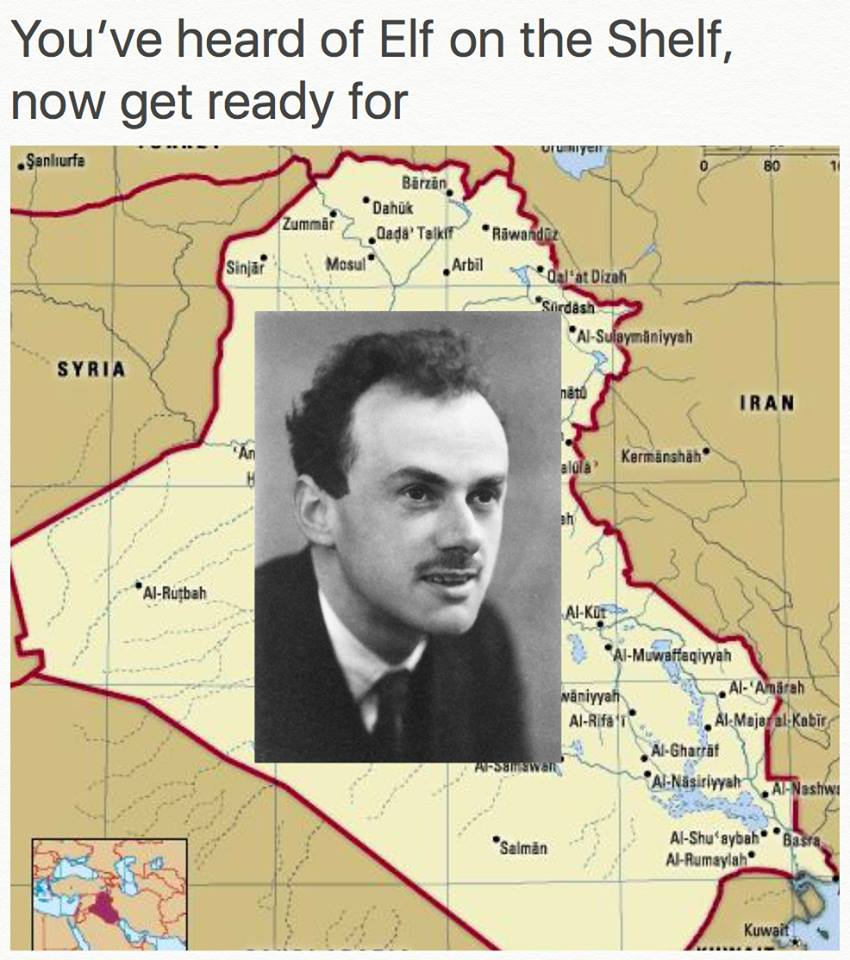
\includegraphics[width=0.6\textwidth]{mech_cover}

  \vspace{5mm}

  \textbf{\Huge{Level Two Physics: Mechanics}}
\end{center}

\vspace{5mm}

\noindent
\large{There are three questions, worth a total of \numpoints\ marks.\\
       Attempt ALL questions, showing all working.\\
       Read questions carefully before attempting them.\\
       Marks are available for partial answers.\\
       The amount of time expected to be spent per question may not necessarily correlate ``nicely'' to the number of marks.\\
       Diagrams may be used to support answers.\\
       Candidates who do not provide diagrams for some questions may be disadvantaged.\\
       Some marks are given for clarity and neatness of solutions or proofs.}
\vspace{2mm}

\vfill

\begin{flushright}
  \begin{tabular}{ll}
    \textbf{Time Allowed:}& One Hour\\
    \textbf{Achieved:}& 9 marks\\
    \textbf{Merit:}& 14 marks\\
    \textbf{Excellence:}& 20 marks
  \end{tabular}

  \gradetable[v][questions]
\end{flushright}

\end{coverpages}

\begin{questions}
  \titledquestion{The Trampoline}
    \begin{parts}
      \part[2] An object of mass \SI{3.0}{\kilo\gram} is lifted \SI{30}{\metre} above a trampoline. How much gravitational potential
            energy is gained by the object?
      \part[3] The object is dropped; when it hits the trampoline, the elastic surface is depressed by \SI{30}{\centi\metre}. What is the
            spring constant $ k $ of the trampoline?
      \part Another object of mass $ M $ is moving with velocity $ v $ when it hits the same trampoline.
        \begin{subparts}
          \subpart[2] Show that $ x = \sqrt{\frac{Mv^2}{k}} $, where $ x $ is the displacement of the trampoline surface on impact.
          \subpart[1] The object is of mass $ M = \SI{2.0}{\kilo\gram} $ and the trampoline is depressed by \SI{2}{\centi\metre}. How
                   fast was the object moving?
        \end{subparts}
    \end{parts}
  \titledquestion{Feel the Force}
    \begin{parts}
      \part[3] Two cars (red and blue) collide as shown in the diagram (not to scale) and stick together. The angle between the two vectors is \SI{30}{\degree}.

            \begin{center}
              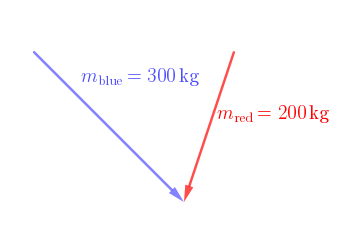
\includegraphics[width=0.4\textwidth]{momentum1}
            \end{center}

            The magnitude of the momentum of the combined mass is \SI{1.0e4}{\kilo\gram\metre\per\second}. The red
            car was initially travelling at a speed of \SI{30}{\metre\per\second}. What was the initial speed of the
            blue car?
      \part A small child swings a ball at a constant speed around his head. The mass of the ball is \SI{0.5}{\kilo\gram}, and the string is of
            length \SI{1.1}{\metre}. The total tension in the string is \SI{20}{\newton}.
        \begin{subparts}
          \subpart[2] Draw a force diagram showing the gravitational, centripetal, and tension forces.
          \subpart[3] Find the magnitude of the centripetal force, and hence calculate the speed of the ball.
        \end{subparts}
    \end{parts}
  \titledquestion{Cannons and Cars}
    \begin{parts}
      \part A cannon shoots a ball at an initial velocity of \SI{3.0}{\metre\per\second}, and the ball travels a total distance
            of \SI{30}{\metre} measured along the ground.
        \begin{subparts}
          \subpart[1] What assumptions must we make in order to model the ball as a projectile?
          \subpart[3] What was the angle of the cannon when the ball was fired?
        \end{subparts}
      \part A toy car is released at a velocity of \SI{1.0}{\metre\per\second}, and takes \SI{10}{\metre} to come
            to a complete halt.
      \begin{subparts}
        \subpart[1] Compute the time taken for the car to come to a stop.
        \subpart[3] The mass of the car is \SI{0.2}{\kilo\gram}. How much energy is dissipated by friction in the first three seconds of the car's motion?
      \end{subparts}
    \end{parts}
\end{questions}

\end{document}
